% This is "sig-alternate.tex" V2.0 May 2012
% This file should be compiled with V2.5 of "sig-alternate.cls" May 2012
%
% This example file demonstrates the use of the 'sig-alternate.cls'
% V2.5 LaTeX2e document class file. It is for those submitting
% articles to ACM Conference Proceedings WHO DO NOT WISH TO
% STRICTLY ADHERE TO THE SIGS (PUBS-BOARD-ENDORSED) STYLE.
% The 'sig-alternate.cls' file will produce a similar-looking,
% albeit, 'tighter' paper resulting in, invariably, fewer pages.
%
% ----------------------------------------------------------------------------------------------------------------
% This .tex file (and associated .cls V2.5) produces:
%       1) The Permission Statement
%       2) The Conference (location) Info information
%       3) The Copyright Line with ACM data
%       4) NO page numbers
%
% as against the acm_proc_article-sp.cls file which
% DOES NOT produce 1) thru' 3) above.
%
% Using 'sig-alternate.cls' you have control, however, from within
% the source .tex file, over both the CopyrightYear
% (defaulted to 200X) and the ACM Copyright Data
% (defaulted to X-XXXXX-XX-X/XX/XX).
% e.g.
% \CopyrightYear{2007} will cause 2007 to appear in the copyright line.
% \crdata{0-12345-67-8/90/12} will cause 0-12345-67-8/90/12 to appear in the copyright line.
%
% ---------------------------------------------------------------------------------------------------------------
% This .tex source is an example which *does* use
% the .bib file (from which the .bbl file % is produced).
% REMEMBER HOWEVER: After having produced the .bbl file,
% and prior to final submission, you *NEED* to 'insert'
% your .bbl file into your source .tex file so as to provide
% ONE 'self-contained' source file.
%
% ================= IF YOU HAVE QUESTIONS =======================
% Questions regarding the SIGS styles, SIGS policies and
% procedures, Conferences etc. should be sent to
% Adrienne Griscti (griscti@acm.org)
%
% Technical questions _only_ to
% Gerald Murray (murray@hq.acm.org)
% ===============================================================
%
% For tracking purposes - this is V2.0 - May 2012

\documentclass{sig-alternate}

\usepackage{graphicx}
\usepackage{caption}
\usepackage{subcaption}

\begin{document}
%
% --- Author Metadata here ---
\conferenceinfo{WOODSTOCK}{'97 El Paso, Texas USA}
%\CopyrightYear{2007} % Allows default copyright year (20XX) to be over-ridden - IF NEED BE.
%\crdata{0-12345-67-8/90/01}  % Allows default copyright data (0-89791-88-6/97/05) to be over-ridden - IF NEED BE.
% --- End of Author Metadata ---

\title{Recognition of Continuous Gestures with Dynamic Hand Pose and Path for
Mid-Air Interaction}
%
% You need the command \numberofauthors to handle the 'placement
% and alignment' of the authors beneath the title.
%
% For aesthetic reasons, we recommend 'three authors at a time'
% i.e. three 'name/affiliation blocks' be placed beneath the title.
%
% NOTE: You are NOT restricted in how many 'rows' of
% "name/affiliations" may appear. We just ask that you restrict
% the number of 'columns' to three.
%
% Because of the available 'opening page real-estate'
% we ask you to refrain from putting more than six authors
% (two rows with three columns) beneath the article title.
% More than six makes the first-page appear very cluttered indeed.
%
% Use the \alignauthor commands to handle the names
% and affiliations for an 'aesthetic maximum' of six authors.
% Add names, affiliations, addresses for
% the seventh etc. author(s) as the argument for the
% \additionalauthors command.
% These 'additional authors' will be output/set for you
% without further effort on your part as the last section in
% the body of your article BEFORE References or any Appendices.

\numberofauthors{2} %  in this sample file, there are a *total*
% of EIGHT authors. SIX appear on the 'first-page' (for formatting
% reasons) and the remaining two appear in the \additionalauthors section.
%
\author{
% You can go ahead and credit any number of authors here,
% e.g. one 'row of three' or two rows (consisting of one row of three
% and a second row of one, two or three).
%
% The command \alignauthor (no curly braces needed) should
% precede each author name, affiliation/snail-mail address and
% e-mail address. Additionally, tag each line of
% affiliation/address with \affaddr, and tag the
% e-mail address with \email.
%
% 1st. author
\alignauthor
Ying Yin\\
       \affaddr{Massachusetts Institute of Technology}\\
       \affaddr{}\\
       \affaddr{}\\
       \email{yingyin@csail.mit.edu}
% 2nd. author
\alignauthor
Randall Davis \\
       \affaddr{Massachusetts Institute of Technology}\\
       \affaddr{}\\
       \affaddr{}\\
       \email{davis@csail.mit.edu}
}

\maketitle
\begin{abstract}
We explored different hand pose features for recognition of continuous gestures
with dynamic hand pose and path. We use Abstract Hidden Markov Model (AHMM)
which handles gesture segmentation and transition inherently within the model.
\end{abstract}

%A category including the fourth, optional field follows...
\category{H.5.2}{Information Systems}{Information Interfaces and
Presentation}[User Interfaces]

\keywords{Continuous gesture recognition, AHMM, HOG}

\section{Introduction}
Gesture can be an important modality for a multimodal interaction system.
With large number of joints, our hands are very expressive. We use our hands to
manipulate objects and communicate ideas and sometimes even subconsciously. This
also makes gesture recognition a hard problem because gestures are less
structured compared to speech.

\section{Related Work}
Wobbrock et al. \cite{Wobbrock09} identified 6 \textit{forms} of gesture for surface
interaction: static pose, dynamic pose,
static pose and path, dynamic pose and path, one-point touch, and one-point
path. One-point touch and one-point path are just special cases for static pose
and static pose and path respectively and are most relevant for surface
interaction. We consolidate that for mid-air interaction
(Table~\ref{tab:gesture-form}).
Among them, the dynamic pose and path gestures are the most complicated ones. 

\begin{table}
\centering
\caption{Gesture form taxonomy}
\begin{tabular}{|l|l|} \hline
\textbf{Gesture Form}&\textbf{Explanation}\\ \hline
static pose & Hand pose is held in one location. \\ \hline
dynamic pose & Hand pose changes in one location. \\ \hline
static pose and path & Hand pose is held as hand moves. \\ \hline
dynamic pose and path & Hand pose changes as hand moves. \\
\hline\end{tabular}
\label{tab:gesture-form}
\end{table}

HOG (histograms of oriented gradients) feature \cite{dalal05} is used widely
in object recognition with great success. It is often used with a linear SVM
classifier. It was originally used in pedestrian recognition and is also used in 
gesture recognition \cite{song12}. In particular, Song et al. used a SVM
classifier with HOG feature derived from the hand image to classify different
static hand poses in their gesture set and use the probability output . Their
data set contains gestures with static hand pose and path but not dynamic hand pose and path. While it is easier
to identify classes of static hand poses with ground truth labels and train a
classifier using supervised learning, it is harder to do so with dynamic hand
poses as hand poses change continuously. In this paper, we explore unsupervised
clustering method with different hand pose features for our 


\section{Recognition of Continuous Gesture with Dynamic Hand Poses}
We use Abstract Hidden Markov Model (AHMM) to model gesture production, and
develop a learning and predication framework based on this model.

\subsection{Hand Tracking Using a RGB-D Camera}
The RGB-D(epth) camera such as the Kinect is a relatively cheap sensor for 
body motion tracking which can used in everyday applications. Camera-based
sensors are also less obtrusive as users do not need to wear any additional
devices. The depth camera is less sensitive to lighting conditions than the RGB
camera but the RGB camera can still provide some additional information to
further improve the tracking accuracy.

As we are interested in gestures with both dynamic path and hand poses, we want
to extract hand pose features for our recognition engine. As a first step, we
consider gestures using left hand only.

We use the Microsoft Kinect SDK for user detection and skeleton tracking. The
skeleton tracking is based on depth information and tracks 20 body joints
including the both hand joints.
We notice that while the skeleton tracking works well for articulated body poses,
it fails to track hand joints correctly when the hands are close to and in
front of the body or the hand movement is fast (see Figure~\ref{fig:skin} for
some examples of such failure).

\begin{figure*}
\centering
\begin{subfigure}{0.485\textwidth}
  \centering
  \includegraphics[height=0.35\columnwidth]{fig/rest.ps}
  \caption{Rest position}
\end{subfigure}
\begin{subfigure}{0.485\textwidth}
  \centering
  \includegraphics[height=0.35\columnwidth]{fig/shakehand.ps}
  \caption{Shake hand}
\end{subfigure}
\caption{Examples when skeleton tracking fails.}
\label{fig:skin}
\end{figure*}

To improve the hand tracking result we use the RGB camera information for skin
detection. We convert the RGB image i into YCrCb color space and perform a
binary classification of each pixel. We filter out the wrongly detected skin
region (background or objects with colors similar to skin color) by finding the
intersection between the skin mask and the user mask. Then we find the contours
with perimeter that is greater than the minimum possible hand shape. This
results in contours for the head and two hands and possible other contours due
to wrong skin region close to the body. To find the most probable contour for
the left hand, we consider the Euclidean distances from the center of each
contour, $\bf{c}_i$, to the left hand joint position from skeleton
tracking, , $\bf{h}_S$, and the previous left hand position, $\bf{h}_P$. We rank
the contours with a cost metric
\begin{displaymath}
\text{Cost}(\bf{c}_i) = w_1 \cdot ||\bf{c}_i - \bf{h}_S|| + w_2 \cdot ||\bf{c}_i
- \bf{h}_P||
\end{displaymath}
All positions are in the depth image coordinates. The final left hand contour is
the one with the lowest cost.
The two weights $w_1$ and $w_2$ control the relative importance of the two distances. The
skeleton tracking also returns the the confidence of the tracking results in two
levels: \textit{tracked} (high confidence) and \textit{inferred} (low
confidence). While keeping $w_2 = 1$, we adjust $w_1$ according to the skeleton
tracking confidence
\begin{displaymath}
w_1 = 
\begin{cases}
  1, & \text{if } \bf{h}_S \text{ is tracked} \\
  0.25, & \text{if } \bf{h}_S \text{ is inferred} 
\end{cases}
\end{displaymath}
Starting from the bounding box of the most likely left hand
contour, we use CamShift \cite{Bradski98} on the depth mapped image
to locate the final bounding box of the hand. Figure~\ref{fig:skin} shows
examples of final tracked left hand.

\subsection{Continuous Gesture Recognition Framework}
We use the 1-level abstract hidden Markov model (AHMM)
proposed by Bui et al.~\cite{bui00} for continuous gesture recognition because
it maps closely to the gesture production process. 

\begin{figure}
\centering
\epsfig{file=fig/ahmm.eps}
\caption{Dynamic Bayesian network representation of 1-level AHMM}
\label{fig:ahmm}
\end{figure}


\subsubsection{The Model}
The AHMM model is closely related to hierarchical hidden Markov models (HHMMs).
HHMMs is an extension of the HMM that is designed to model domains with
hierarchical structure and/or dependencies at multiple length/time
scales~\cite{murphy02}. Each gesture can be modeled by an HMM with variable
length as users make gestures with changing speed. A sequence of gestures can
then be viewed as a hierarchy of HMMs. 

Figure~\ref{fig:ahmm} shows the 1-level AHMM we use for gesture recognition 
represented in a dynamic Bayesian network (DBN). Node
$G_t$ represents the gesture that the
gesturer is making at time $t$. It can include different gestures the system
can recognize as well as rest poses and pre- and post-gesture strokes.
Node $S_t$ is the hidden state of the hand movement, which is essentially a
vector quantization of the actual, observed (but noisy) feature vector $X_t$. 
Node $F_t^G$ is a binary variable that indicates the end of a
gesture. It is ``on'' (has value 1) if the lower level HMM at time $t$ has just
``finished'', otherwise it is ``off'' (value 0). Thus, the use of node $F_t^G$
incorporates gesture segmentation into the probabilistic model seamlessly. We
do not need a separate mechanism to do gesture segmentation and then use HMM for
gesture recognition. It is also probabilistic and hence can be more robust.

One difference between this 1-level AHMM and a general HHMM is that state $S$ never
``resets'', since $F^G$ is not a parent. Here we assume that during a gesture sequence, even if the goal changes,
the next state of the hand/arm movement always depends on the previous state. This is reasonable for gesture recognition because the hand/arm 
movement is always continuous, unless the hands move out of the sensor's view during
which the inference engine will reset. 

\subsubsection{Hand Feature}
We combine both hand motion features, $X^M_t$ and hand pose features, $X^P_t$
for the observation node $X_t$, i.e., 
\begin{displaymath}
X_t = \left[X^M_t\right]
\end{displaymath} 

The motions features include the relative position of the center of
the hand bounding box $\bf{p}$, velocity $\bf{v}$ and acceleration $\bf{a}$.
All of them are 3-dimensional vectors in the world
coordinate system.

The hand pose features are computed from a $100 \times 100$ px image $I$ scaled
from the bounding box of the final tracked left hand (Figure~\ref{}). Each pixel
is a depth value scaled between $0$ and $255$. We explore several hand pose 
features derived from the image.

\begin{figure}

\end{figure}

\subsubsection{Eigenhand}
This is similar to the eigenface~\cite{turk91} technique. We concatenate the
rows of the hand image, $I$, into one one column vector and perform principle
component analysis (PCA) on all the training images. The images
reshaped from the eigenvectors are the eigenhands (Figure~\ref{}). We use
the first $n$ eigenvectors, $u_1, \ldots, u_n$, corresponding to the 
$n$ largest eigenvalues as our basis.
Hence, the hand pose feature vector is a $n$-dimensional vector $[w_1,
\ldots, w_n]$ where each component is the projection of the hand into each
eigenvectors $u_1, \ldots, u_n$.

\begin{figure}

\end{figure}

\subsubsection{HOG}


\section{Experimental Evaluation}
We evaluate our hand tracking and gesture recognition algorithm with part of the ChAirGest 
dataset. We use two session 4 subjects and 10 gestures and 3 resting postures.  
There are 2 occurrences for each gesture/resting posture per subject. So overall 
there are 600 gesture occurrences. For each user, we use 2 sessions of recording. 
In each session there are one occurrence for each gesture/resting posture combination 
resulting in 30 gesture occurrences. We use one session for training and one session for testing.

The RGB and depth videos are 30 fps (frame per second) and we down sample them
to 10 fps to increase training speed.

\section{Future Work}
We note that our method of combining skin color detection, user detection and
skeleton tracking can fail when the user is wearing clothes with color similar
to the skin color. Consider use a probability distribution of skin color instead
of binary classification. Consider use STIP feature. Track two hands or consider
features for the whole body. 

\section{Conclusions}

%\end{document}  % This is where a 'short' article might terminate

%ACKNOWLEDGMENTS are optional
\section{Acknowledgments}

%
% The following two commands are all you need in the
% initial runs of your .tex file to
% produce the bibliography for the citations in your paper.
\bibliographystyle{abbrv}
\bibliography{sigproc}  % sigproc.bib is the name of the Bibliography in this case
% You must have a proper ".bib" file
%  and remember to run:
% latex bibtex latex latex
% to resolve all references
%

%\balancecolumns % GM June 2007
% That's all folks!
\end{document}
